\section{Particles and Interactions in the Standard Model}

The Standard Model, shown in~\Cref{fig:sm_particles}, consists of 12 elementary
spin-$\frac{1}{2}$ particles referred to as \emph{fermions} and their
anti-particles, and five types of particles with integer spin referred to as
\emph{bosons}. With the discovery of the Higgs boson in
2012~\cite{HIGG-2012-27,CMS-HIG-12-028}, experimental evidence for the existence
of all fermions and bosons predicted by the Standard Model is established.

\begin{figure}[htbp]
  \centering

  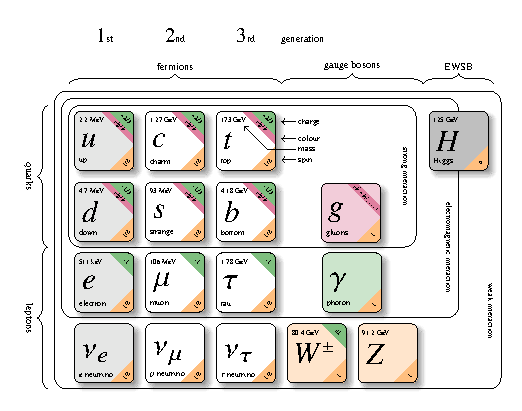
\includegraphics[width=\textwidth]{theory/sm}

  \caption{Particles of the SM. The diagram is adapted from Ref.~\cite{sm_tikz}
    with updated particle properties from Ref.~X. Antiparticles are not shown
    explicitly have additive quantum numbers of opposite sign but otherwise the
    same properties of the respective particle.}
  \label{fig:sm_particles}
\end{figure}


The elementary particles of the SM can be divided into three categories:
\begin{description}

\item[Fermions] predicted by the SM have spin-$\frac{1}{2}$. Consequently, they
  are massive\footnote{Neutrinos are considered as massless in the SM, however,
    the observation of neutrino
    oscillations~\cite{Super-Kamiokande:1998kpq,SNO:2002tuh} is experimental
    evidence for neutrinos having small but non-zero mass.} and adhere to the
  Pauli exclusion principle and are therefore considered to be \emph{matter}
  particles. For every fermions, a corresponding anti-particle exists that has
  the same properties but with opposite additive quantum numbers. The fermions
  of the SM are divided into \emph{quarks} that take part in the strong
  interaction and \emph{leptons} that do not. They are further divided into
  up-type quarks ($u$, $c$, $t$), down-type quarks ($d$, $s$, $b$), charged
  leptons ($e$, $\mu$, $\tau$), and neutrinos ($\nu_e$, $\nu_\mu$,
  $\nu_\tau$). The fermions of the SM come in three generations, the main
  difference between them being the mass of the fermions. All ordinary (stable)
  matter consists of fermions of the first generation: up-quarks, down-quarks,
  and electrons.

  The fermions carry charge-like quantum numbers that dictate the fundamental
  interactions they take part in. Quarks carry \emph{colour charge} which comes
  in three discrete values of either \emph{red}, \emph{green}, or \emph{blue},
  and the corresponding anti-colours for anti-quarks. Particles carrying colour
  charge take part in the strong interaction. Quarks and (electrically) charged
  leptons carry \emph{electric charge} and are therefore subject of the
  electromagnetic interaction. Fermions (anti-fermions) with left-handed
  (right-handed) chirality carry \emph{weak isospin} therefore taking part in
  charged-current weak interactions. All fermions carry \emph{weak hypercharge}
  and therefore take part in neutral current weak interactions.

\item[Gauge bosons] predicted by the SM are particles with spin-$1$ and are
  therefore also referred to as vector bosons. Gauge bosons are the quanta of
  fields arising in theories built on certain symmetry principles, referred to
  as gauge theories, which will discussed in
  \Cref{sec:theo_symmetries_interactions}. The gauge bosons mediate the three
  fundamental forces of nature through particle exchange.

  The (massless) gluons mediate the strong interaction through exchange of
  gluons between particles carrying colour charge. Gluons carry colour charge
  themselves and therefore couple to quarks or other gluons. The (massless)
  photon mediates the electromagnetic interaction between electrically charged
  particles. The gauge bosons of the weak interaction, the $W^\pm$ and $Z$
  bosons, take a special role in the SM since they are the only massive gauge
  bosons. The $W$ bosons are electrically charged and mediate the charged
  current weak interaction between particles carrying weak isospin. The
  uncharged $Z$ boson mediates the neutral-current weak interaction between
  particles carrying weak hypercharge.

\item[The Higgs boson] is the only scalar (spin-$0$ and positive parity)
  particle in the SM. The Higgs boson is a by-product of the
  Brout--Englert--Higgs (BEH) mechanism~\cite{Englert:1964et,Higgs:1964pj} that
  is used to include massive gauge bosons, the $W^\pm$ and $Z$ bosons, in the SM
  without violating the underlying principles of the gauge theory. This will be
  elaborated in \Cref{seq:theory_ewk}.

\end{description}

%%% Local Variables:
%%% mode: latex
%%% TeX-master: "../../phd_thesis"
%%% End:
